\documentclass[a4paper]{article}
\usepackage{graphicx}
\usepackage{xcolor} % Load this before hyperref
\definecolor{softblue}{RGB}{70,130,180}
\usepackage[colorlinks=true, linkcolor=softblue, citecolor=softblue, filecolor=softblue, urlcolor=softblue]{hyperref}

\title{\textbf{Assignment 1:\\Macbook M1 Pro Benchmark}}
\author{
    Yazeed AlKhalaf\\
    \textbf{Course:} CIS 304 - Computer Architecture\\
    \textbf{Instructor:} Dr. Adeel Baig
}
\date{\textbf{Date:} 21 Feb, 2024}

\begin{document}

\maketitle

\newpage

\section{Specs of The Machine}

The machine we are going to run tests on in this experiment is the Macbook Pro with the Apple M1 Pro chip.

Specs:
\begin{itemize}
    \item \textbf{Chip:} Apple M1 Pro @ 3.22 GHz
    \begin{itemize}
        \item \textbf{Total Number of CPU Cores:} 10 (8 performance and 2 efficiency)
        \item \textbf{Total Number of GPU Cores:} 16
        \item \textbf{Total Number of Neural Engine Cores:} 16
    \end{itemize}
    \item \textbf{Memory:} 16GB (LPDDR5 by Samsung)
    \begin{itemize}
        \item \textbf{Memory Bandwidth:} 200GB/s
    \end{itemize}
\end{itemize}

Model Indetifier for reference: \textbf{MacBookPro18,3}

More details can be found on the Apple website: \url{https://support.apple.com/kb/SP854?locale=en_US}

\section{Benchmarking Tools}

In this section, we will be examining the results of the benchamrking tools that stress both the CPU and the GPU.

\subsection{Geekbench (CPU)}

\begin{figure}[h!]
    \centering
    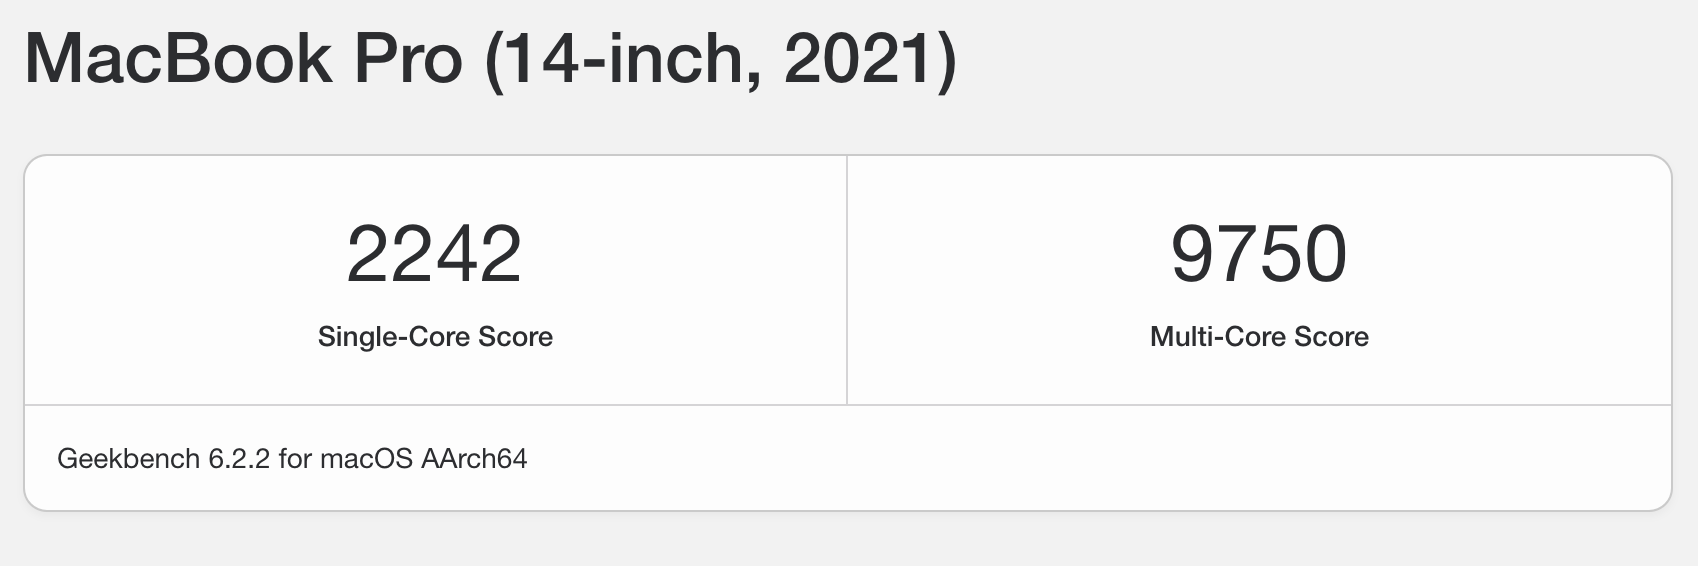
\includegraphics[width=0.8\textwidth]{images/geekbench-single-multi-core.png}
    \caption{Geekbench CPU Single and Multi Core Test Results}
    \label{fig:geekbench-single-multi-core}
\end{figure}

The CPU stress test benchmarks the Apple M1 Pro chip. The results are shown in \textbf{Figure \ref{fig:geekbench-single-multi-core}} and are as follows:

\begin{itemize}
    \item \textbf{Single-Core Score:} 2242
    \item \textbf{Multi-Core Score:} 9750
\end{itemize}

\subsection{Geekbench (GPU)}

The GPU stress test performed by Geekbench on macOS supports two GPU APIs: Metal and OpenCL. We will be examining the results of both.

The results of this test on Geekbench: \url{https://browser.geekbench.com/v6/cpu/5025983}

\subsubsection{Metal}

\begin{figure}[h!]
    \centering
    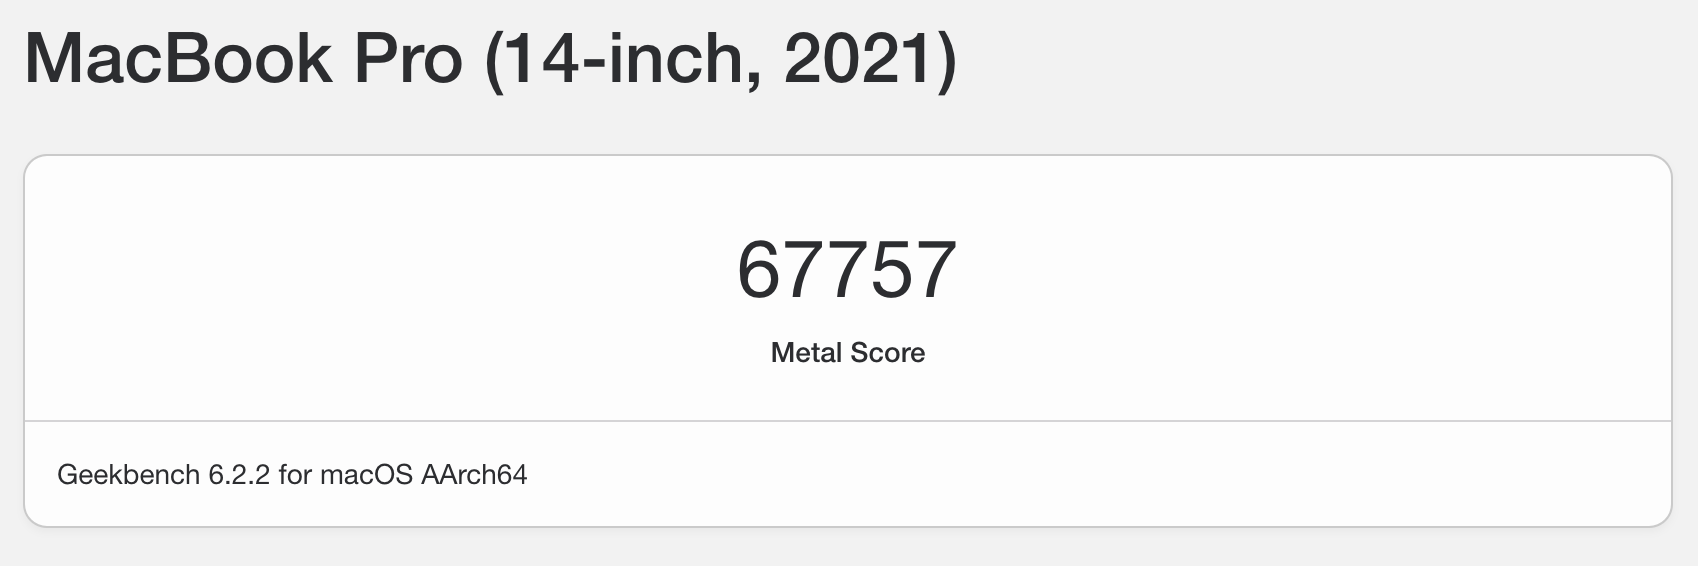
\includegraphics[width=0.8\textwidth]{images/geekbench-gpu-metal.png}
    \caption{Geekbench GPU Metal Test Results}
    \label{fig:geekbench-gpu-metal}
\end{figure}

The GPU stress test benchmarks the Apple M1 Pro chip. The results are shown in \textbf{Figure \ref{fig:geekbench-gpu-metal}} and are as follows:

\begin{itemize}
    \item \textbf{Metal Score:} 67757
\end{itemize}

The results of this test on Geekbench: \url{https://browser.geekbench.com/v6/compute/1805495}

\subsubsection{OpenCL}

\begin{figure}[h!]
    \centering
    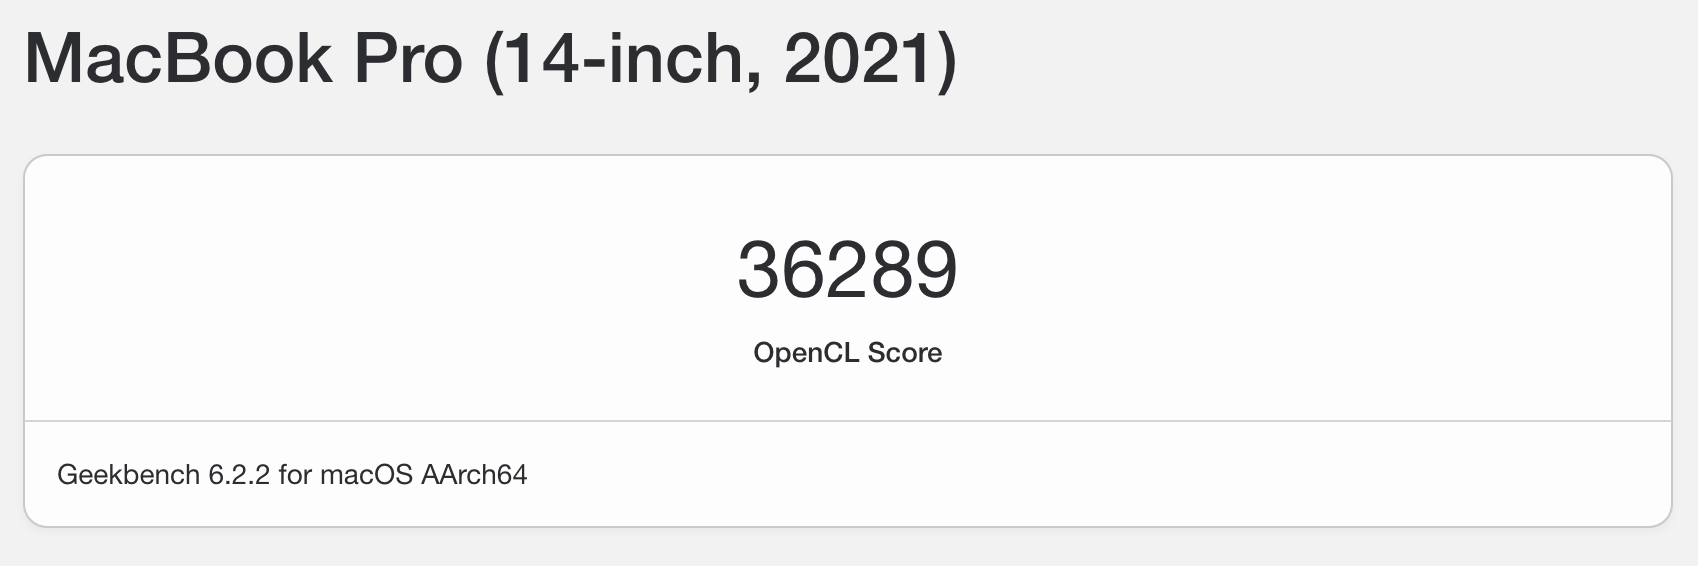
\includegraphics[width=0.8\textwidth]{images/geekbench-gpu-opencl.png}
    \caption{Geekbench GPU OpenCL Test Results}
    \label{fig:geekbench-gpu-opencl}
\end{figure}

The GPU stress test benchmarks the Apple M1 Pro chip. The results are shown in \textbf{Figure \ref{fig:geekbench-gpu-opencl}} and are as follows:

\begin{itemize}
    \item \textbf{OpenCL Score:} 36289
\end{itemize}

The results of this test on Geekbench: \url{https://browser.geekbench.com/v6/compute/1805535}

\subsection{Blackmagic Disk Speed Test}

The disk test by Blackmagic does the following:

\begin{enumerate}
    \item Does the write test which lasts for 8 seconds.
    \item Does the read test which also lasts for 8 seconds.
\end{enumerate}

The total testing time is 16 seconds. The tool keeps on repeating this til you click the big start button in the middle of the guages again.

The tool's website: \url{https://apps.apple.com/us/app/blackmagic-disk-speed-test/id425264550}

\subsubsection{The Test Settings}

\begin{figure}[h!]
    \centering
    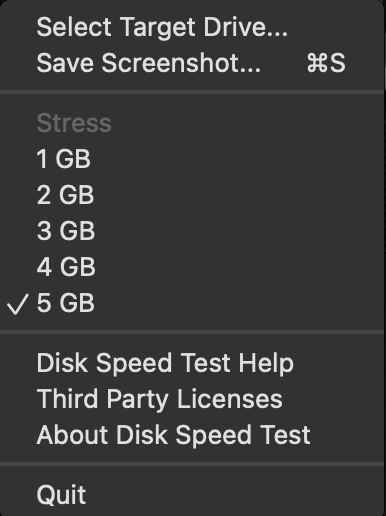
\includegraphics[width=0.5\textwidth]{images/blackmagic-disk-stress-settings.png}
    \caption{Blackmagic Disk Stress Test Settings}
    \label{fig:blackmagic-disk-stress-test-settings}
\end{figure}

The test settings, shown in \textbf{Figure \ref{fig:blackmagic-disk-stress-test-settings}}, are stressing the disk with 5 GB. This is the highest available option in this tool and will show us clearly how the Macbook performs under pressure.

\subsubsection{The Test Results}

\begin{figure}[h!]
    \centering
    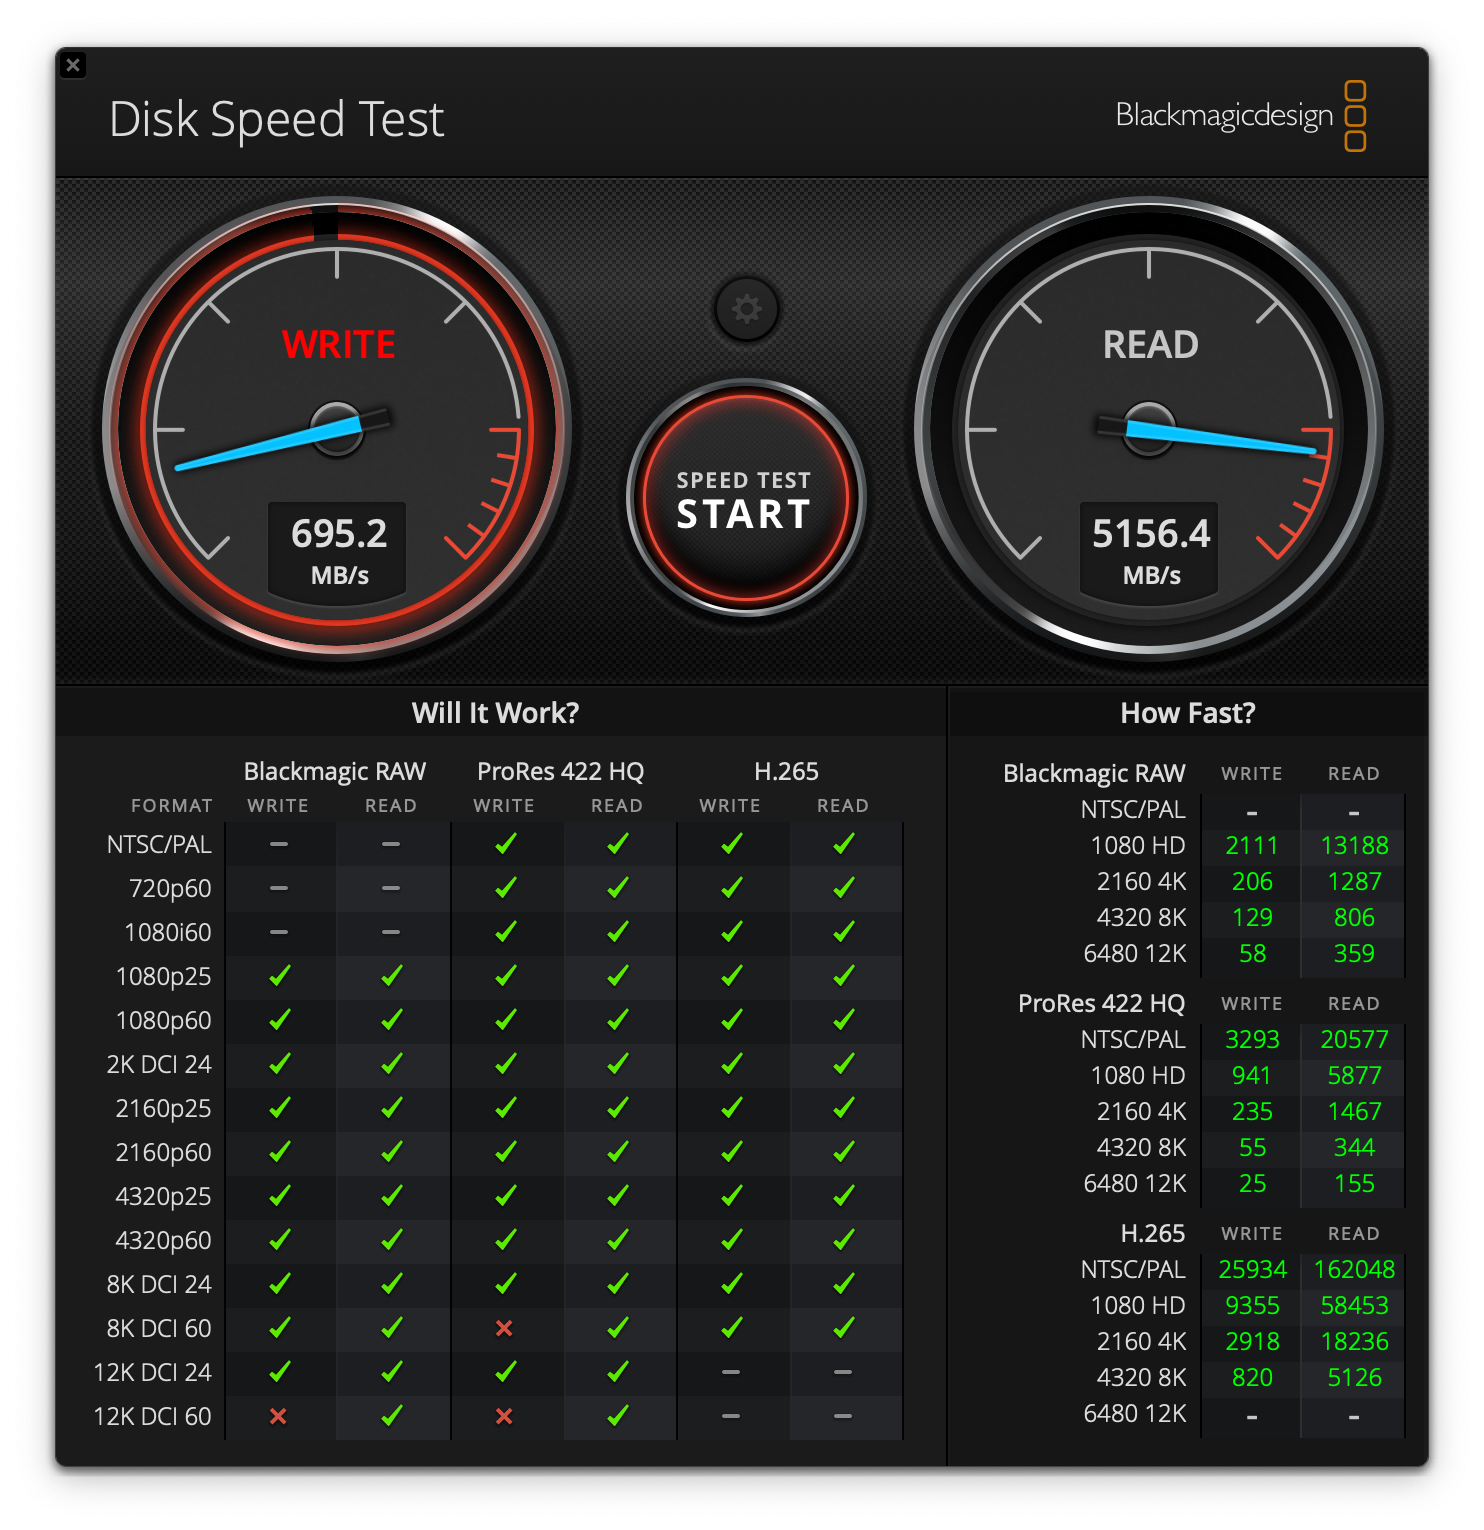
\includegraphics[width=0.5\textwidth]{images/blackmagic-disk-stress-result.png}
    \caption{Blackmagic Disk Stress Result}
    \label{fig:blackmagic-disk-stress-test-result}
\end{figure}

The test results for this disk stress test has two panels:

\begin{enumerate}
    \item \textbf{Will it Work?:} This panel shows which video formats can be supported by your disk storage
    \item \textbf{How Fast?} This panel shows results in frames per second (fps)
\end{enumerate}

The first panel, Will it Work?, is starightforward. It shows a checkmark if your disk supports running this video format.

But for the second panel, How Fast?, it might not be so clear at first. It tells how many frames of a video you can read per second from your disk. If you are editing a video that is 8K at 60fps but your disk can't keep up and maxes out its read of fps at 50, you will get a choppy playback. Also you will struggle to run more than one 8K video simultaneously. Now if you got frames per second that are way more than one video frames per second, then you are good to go. For example, the Macbook I ran the tests on can read 5126 frames per second of (4320 8K video) in the (H.265) format. That should be enough for almost every use case possible with this machine.

\section{Analysis Tool}

TG Pro is a great companion for monitoring the heat of different components of your Macbook. The menu bar icon shows the 

\end{document}